
\section*{Notation and definitions.} The following tools will be used in this paper. Let $K \subseteq \RR^{n}$ be a non empty convex set. The normal cone to $K$ at $x \in \RR^{n}$ is $N_{K}(x)=\{z \in \RR^{n} | \langle z, \zeta-x \rangle \leq 0\;\mbox{for all}\;\zeta \in K\}$. The projection in the euclidean metric of a vector $x \in \RR^{n}$ onto $K$ is denoted as proj$[K;x]$. The identity matrix of $\RR^{m \times m}$ is denoted by $\mathsf I_m$ and the zero vector in $\RR^m$ by $0_m$.
The Mixed Complementarity Problem (MCP)~\cite{Dirkse.Ferris1995}]) is defined as follows. Given a function $\mathsf F : \RR^p \rightarrow \RR^p$, lower and
  upper bounds $l, u \in (\RR \cup \{+\infty, -\infty\})^p$, find $z \in \RR^{p}$, $w,  v \in \RR^{p}_{+}$, such that
  \begin{equation*}\label{eq:MCP}
      \begin{array}{l}  
        \mathsf F(z) = w-v 
        l \leq z \leq u, 
        (z-l)^{T}w=0,
        (u-z)^{T}v=0,
      \end{array}
  \end{equation*}
which implies $-F(z) \in N_{[l,u]}(z)$.
 If the $\mathsf F(z) = M z +q$ in (\ref{eq:MCP}) 
for some matrix $M \in \RR^{ p \times p}$ and some vector $q\in\RR^m$, the MCP~(\ref{eq:MCP}) defines a  Mixed Linear Complementarity Problem (MLCP).


\section{Introduction}
\textcolor{navyblue}{\IEEEPARstart{I}{t} is well know that conventional accurate analog simulation tools, which are based on the Newton--Raphson nonlinear solver, can have serious drawbacks when they are used for the integration of switched circuits, containing switches and piecewise linear components (like ideal diodes and transistors). Then analog ({\sc Spice}-like) tools  may become very time consuming, or provide very poor results with chattering \cite{galias2006}, or even fail \cite{maffezzoni2006,yuan2003,mayaram2000,chung1994,biolek2007}. The same applies to ``hybrid'' integrators that consider an exhaustive enumeration of all the system's modes, which have a very limited scope of application because of the exponential growth of the number of modes that have to be simulated separately. Along the same lines, event-driven schemes can hardly simulate systems with large number of events, because they soon become quite time-consuming and do not allow for accumulations of events \cite{acary-brogliato2008}. }

The objective of this paper is twofold: firstly it is shown on an academic example taken from \cite{maffezzoni2006} that the NSDS approach allows one to simulate a nonsmooth system for which conventional analog methods fail (roughly speaking, the iterative solver for complementarity problems converges, whereas Newton-Raphson's method does not); secondly, numerical results for a buck converter are presented and comparisons with other (analog and hybrid) tools are done.  Compared to previous works \cite{glocker2005,vasca2009}, the ideal switches are here modelled and simulated for the first time in a completely implicit way, the advantage of which will be explained.  


\section{The nonsmooth approach for switched circuits.}
\label{section2}

\subsection{Modelling aspects of nonsmooth components}
\label{section21}

 Let us illustrate the nonsmooth modeling on the above two examples (ideal diode, switch).
 \renewcommand{\labelenumi}{\alph{enumi})}
\subsubsection{nonsmooth  diodes}  The notation for the currents and the potentials at the ports of the diode is depicted in Fig.~\ref{fig:DIODE}. Four models of diodes are depicted in Fig.~\ref{figdiodes}:\\
a)the smooth exponential Shockley model in Fig.~\ref{figdiodes-shockley} defined by the smooth constitutive equation,
  \begin{equation}
    \label{eq:diode-shockley}
     i(t) = i_s \exp(- \frac{v(t)}{\alpha} - 1),
  \end{equation}
where $i_s$ and $\alpha$ are physical parameters of the diode,\\
b) ideal diodes with possible residual current $-a$ and voltage $-b$ in Fig.~\ref{figdiodes-complementarity} defined by the following complementarity condition
  \begin{equation}
    \label{eq:diode-complementarity}
     0\leq i(t)+a \perp v(t)+b \geq 0 ,
  \end{equation}
where the $x \perp y $ means that $x^T y =0$ and $a$ and $b$ are the threshold values for $i$ and $v$,\\
c)the ``hybrid'' model which considers the two modes separately with for instance  an associated Modelica~\cite{elmqvist2001} script in Fig.~\ref{figdiodes-hybrid}
  \begin{equation}
    \label{eq:diode-hybrid}
    \begin{array}{cll}
          \mathsf{off} &=& \mathsf{s} < 0 \\
          v(t)  &=& \mathbf{if}\quad \mathsf{off} \quad \mathbf{then}\quad \mathsf{-s} \quad \mathbf{else} \quad 0 \\
          \ i(t) &=& \mathbf{if}\quad \mathsf{off} \quad
          \mathbf{then}\quad 0  \quad \mathbf{else}\quad \mathsf{s},
        \end{array} 
  \end{equation}\\
d) a piecewise-linear model in Fig.~\ref{figdiodes-pwl} defined by
  \begin{equation}
    \label{eq:diode-pwl}
    v(t)=\begin{cases}-R_\on\; i(t) & \mbox{if}\;v(t) < 0 \\   -R_\off\; i(t) & \mbox{if}\;v(t) \geq  0 \\ \end{cases},
  \end{equation}
with $R_\on \ll 1 $ and $ R_\off \gg 1 $ are the  equivalent resistive values of each branches.

 The ideal diode model in Fig.~\ref{figdiodes-complementarity} is chosen in this paper. The drawbacks of the Shockley law is that it introduces high stiffness in the dynamical equations. The hybrid model becomes rapidly unusable if the number $m$ of diodes increases, since the number of modes to be described in the associated script varies as $2^{m}$. The model \ref{figdiodes-pwl} leads a badly conditioned complementarity problems. On the contrary the ideal model of Fig.~\ref{figdiodes-complementarity} yields, when introduced in the dynamics, well-conditioned one, that yield time-stepping methods for which efficient solvers exist.
\begin{figure}
  \centering
  \input{./figure/diode.pstex_t}
  \caption{Diode symbol.}
  \label{fig:DIODE}
\end{figure}

\begin{figure*}[!ht]
  \subfigure[smooth modeling ]{\label{figdiodes-shockley}
        \resizebox{0.22\linewidth}{!}{\input{./figure/shockleylaw.pstex_t}}
  }\hspace{-2mm}
  \subfigure[nonsmooth modeling]  
  {\label{figdiodes-complementarity} 
        \resizebox{0.22\linewidth}{!}{\input{./figure/figdiode.pstex_t}}
  } \hspace{-2mm}
  \subfigure
  [hybrid modelling 
  ]
  {\label{figdiodes-hybrid} % 
        \resizebox{0.26\linewidth}{!}{\input{./figure/hybrid_diode.pstex_t}}
}
  \subfigure[equivalent resistor model]{\label{figdiodes-pwl}
        \resizebox{0.20\linewidth}{!}{\input{./figure/diodeReq.pstex_t}}} 
      \caption{Four models of diodes.}
\label{figdiodes}
\end{figure*}
\subsubsection{nonsmooth switches} Depicted on Fig.~\ref{fig:IDEAL_SWITCH}, The switch is defined by 
%%
\begin{equation}\label{switchmodel1}
v(t)=\left\{\begin{array}{ll} R_\off\; i(t) & \mbox{if}\;u_{c}(t) < 0 \\   R_\on\; i(t) & \mbox{if}\;u_{c}(t) \geq  0  \end{array}\right.
\end{equation} 
%%
where the voltage $u_{c}(\cdot)$ is a state variable of the overall dynamical system, $v(\cdot)$ is the voltage of the switch and $i(\cdot)$ is the current through the switch. The resistors $R_\off \gg 1$ and $R_\on \ll 1$ are chosen by the designer. The switch in (\ref{switchmodel1}) is modeled as follows:
%%
\begin{equation}
  \label{eq:63switch}
\left\{\begin{array}{l}
v(t)=\frac{1}{2}(1+\tau(t))R_\on i(t)+\frac{1}{2}(1-\tau(t))R_\off i(t)  \\ \\ \tau(t) \in \mbox{sgn}(u_{c}(t)) \; \Leftrightarrow \; u_{c}(t) \in -N_{[-1,1]}(\tau(t))
\end{array}\right.
\end{equation}
 It is noteworthy that the voltage $v(t)$ in~(\ref{switchmodel1}) is discontinuous at $u_{c}(t)=0$ for any $i(t) \not = 0$, the jump magnitude being equal to $|(R_\off-R_\on)i(t)|$. The choice that is made in (\ref{eq:63switch}) implies that the discontinuities are ``filled-in'' and the model is consequently multivalued at $u_{c}(t)=0$,  $i(t) \not = 0$. This is precisely what allows one to smoothly simulate the sliding-modes \cite{Acary.Brogliato2009}. 
\begin{figure}
  \centering
  \scalebox{0.7}{
  \input{./figure/IdealSwitch.pstex_t}
  }
  \caption{Ideal switch symbol.}
  \label{fig:IDEAL_SWITCH}
\end{figure}
Let us conclude this section by a generic form of nonsmooth components as
\begin{equation}
  \label{eq:nonsmooth}
   0 \in y + N_K(\lambda)
\end{equation}
where $y$ and $\lambda$ plays the role of slackness (non necessary physical) variables for describing the complete multi--valued behavior of the component. More complex examples and more generic formulation of nonsmooth components can be found in~\cite{Acary.ea_RR2009}.


\subsection{The dynamical equations and their Automatic generation}
\label{sec:acef}
 There are a lot of methods to build a smooth DAE formulation of standard electrical circuits. To cite a few of them, the Sparse Tableau Analysis (STA) and the modified Nodal Analysis (MNA) are the most widespread. An automatic circuit equation generation system extending the MNA has been developed at the INRIA, see the patent \cite{brevet} yielding to the suitable following formulation
\begin{equation}
  \label{eq:SEDGE}
\left\{  \begin{array}{r l}
      \left.\begin{array}{cl}
        \dot x 
               & = f_1(x,z,t) + U(t) \\
            0   & =  f_2(x,z,t)
      \end{array}\right]
    &
    \begin{array}{l}
      \text{\small Semi-Explicit DAE}
    \end{array}
    \\[1mm]
  \left.\begin{array}{cl}
0 &= h(x,z,\lambda,t)\quad\quad\,\\
y &= g(x,z,\lambda,t)\\
  \end{array}\right] & \begin{array}{l}
   \text{\small Input/output relations on}\\
   \text{\small  nonsmooth components}
  \end{array} \\[1mm]
  \left.\begin{array}{l}
  0 \in y + N_K(\lambda)\quad\quad
\end{array}\right.
& \text{ \small "Inclusion rule"}\\
\end{array}\right.
\end{equation}
where $x \in \RR^n$ corresponds to the current in the inductive branches and the voltages in the capacitive branches, $z\in \RR^p$ collects all the node potentials, the currents in the voltage--defined and non--smooth branches and the currents in a subset of the capacitive branches. The choice and the construction of the latter subset of branches is described in details in~\cite{brevet}.  Starting from~(\ref{eq:SEDGE}), the numerical time--discretiation is an extension of the Moreau's time stepping scheme\cite{Moreau1977} which is given by,
\begin{equation}
  \label{eq:SEDGE-discrete}
  \left\{{  
      \begin{array}{l }
        x_{k+1}- x_{k} 
        = h f_1(x_{k+\theta},z_{k+\theta},t_{k+1}) + h U(t_{k+\theta}) \\
        0    =  f_2(x_{k+1},z_{k+1},t_{k+1})
        \\[2mm]
        0 = h(x_{k+1},z_{k+1},\lambda_{k+1},t_{k+1}),\\
        y = g(x_{k+1},z_{k+1},\lambda_{k+1},t_{k+1})\\
        0 \in y_{k+1} + N_K(\lambda_{k+1})
      \end{array}
    }\right. .
\end{equation}

\subsection{Software aspects} From a {\sc Spice} Netlist, the automatic generator builds all the components defined in~(\ref{eq:SEDGE}). The opensource {\sc Siconos/Kernel} library performs the time-discretization following the Moreau time--stepping scheme~(\ref{eq:SEDGE-discrete}) and formulates at each time--step one instance of the associated MCP. The numerical algorithms for the latter problem are in the opensource {\sc Siconos/Numerics} library. The output of the simulation is a file containing the potential and current values in the {\sc Spice} format. The implementation is object-oriented and mainly in C++. The open-source platform {\sc Siconos}\footnote{http://siconos.gforge.inria.fr/}\cite{acary-brogliato2008,Acary-Perignon2007,mathmod} is under GPL license and can be freely used. The equation generator is under private license and can be obtained freely on demand for an academic use.. 


\section{An elementary switching circuit}
\label{section3}


This section is devoted to the  modelling and the simulation of the circuit in Fig.~\ref{fig:figcircuit1}. In \cite{maffezzoni2006} it is shown that Newton-Raphson based methods fail to converge on such a circuit, with the switch model as in (\ref{switchmodel1}). The diode model is the equivalent resistor model of Fig.~\ref{figdiodes} (d). On the contrary the OSNSP solver correctly behaves on the same model.  
\begin{figure}[h]
  \centering
   \resizebox{\linewidth}{!}{
  \input{./figure/CS_circuit.pstex_t}
  }
  \caption{A simple switched circuit.}
  \label{fig:figcircuit1}
\end{figure}
\subsection{The dynamical system}
\label{section31}
The dynamics of the circuit in Fig.~\ref{fig:figcircuit1} is obtained using the algorithm of automatic circuit equation formulation. Applying the automatic equations generation algorithm leads to the following 9-dimensional state vector: $X=(V_1\;V_2\;V_3\;V_4\;I_L\;I_{03}\;I_{04}\;I_s\;I_d)^{T}$, where the potentials and the currents are depicted on Fig.~\ref{fig:figcircuit1}.  The two nonsmooth devices are the diode and the switch. It yields the following system, that fits within the general framework in (\ref{eq:SEDGE}): for the semi--explicit DAE, we obtain
\begin{equation}
  \label{eq:72}
 \left\{ 
    \begin{array}{lll}
      L  \frac{dI_L}{dt}(t) = V_1(t)-V_2(t) &
      I_d(t)+I_s(t)-I_L(t)=0 \\
      I_L(t)-\frac{V_2(t)}{R}=0&
      I_{03}(t)=0\\
      I_{04}(t)-I_{s}(t)=0&
      V_4(t)=20 ,
      V_3=e(t)\\
\end{array}\right. .
\end{equation}
For the input/output relations on nonsmooth componenents, we get
\begin{equation}
 \left\{ \begin{array}{l}
V_{1}(t)=\frac{1}{2}(\tau_{1}(t)-1)R_\off I_{d}(t)-\frac{1}{2}(\tau_{1}(t)+1) R_\on I_{d}(t) \\ 
\begin{split}
 V_{1}(t)-V_{4}(t)= \frac{1}{2}(1+\tau_{2}(t)) R_\off I_{s}(t)
  \quad\quad \\+\frac{1}{2}(1-\tau_{2}(t)) R_\on I_{s}(t)
\end{split}
  %  0 = V_1(t)-V_4(t)+I_s(t) (\lambda_2+R_\on) \\
  %  0 = V_1(t)+I_d(t)(\lambda_4(t)+R_\on) \\
   % y_1(t) = R_\off-\lambda_2(t)-R_\on\\
   % y_2(t) = V_3(t)-V_2(t)+\lambda_1(t)\\
  %  y_3(t) = R_\off-\lambda_4(t)-R_\on\\
  %  y_4(t) = -V_1(t)+\lambda_3(t) \\
  \end{array} \right. .
\end{equation}
 Finally, the inclusion rule is written as
\begin{equation}
  \left\{\begin{array}{l}
      V_{1}(t) \in - N_{[-1,1]}(\tau_{1}(t)) \\   100(V_{3}(t)-V_{2}(t)) \in -N_{[-1,1]}(\tau_{2}(t))
    \end{array} 
\right. .
\end{equation}

\subsection{Numerical results with {\sc Siconos}}
\label{section32}

The time step has been fixed to $0.1 \micro \second$. Fig.~\ref{fig:SICONOS_SIMU_CS} depicts
the current evolution through the inductor $L$. In \cite{maffezzoni2006}, it has been shown that the
Newton-Raphson algorithm fails when the state of the diode and of the switch changes at $t=t_s$ in
Fig.~\ref{fig:SICONOS_SIMU_CS}. Indeed, the linearization performed at each Newton-Raphson
iteration leads to an oscillation between two incorrect states and never converges to the correct
one. The Newton-Raphson iterations enter into a infinite loop without converging. In the nonsmooth framework, The PATH solver\cite{Dirkse.Ferris1995} for MCP or a semi-smooth Newton method\cite{DeLuca.Facchinei.ea2000}  converges and computes the correct state. In \cite{maffezzoni2006} an event-driven numerical method is proposed to solve the non convergence issue. However it is reliable only if the switching times can be precisely estimated, a shortcoming not encountered  with the NSDS and the  Moreau's time-stepping method. 


\begin{figure*}[!ht]
  \subfigure[{\sc Siconos} simulation ]{\label{fig:SICONOS_SIMU_CS}
        \resizebox{0.5\linewidth}{!}{%GNUPLOT: LaTeX picture with Postscript
\begin{picture}(0,0)%
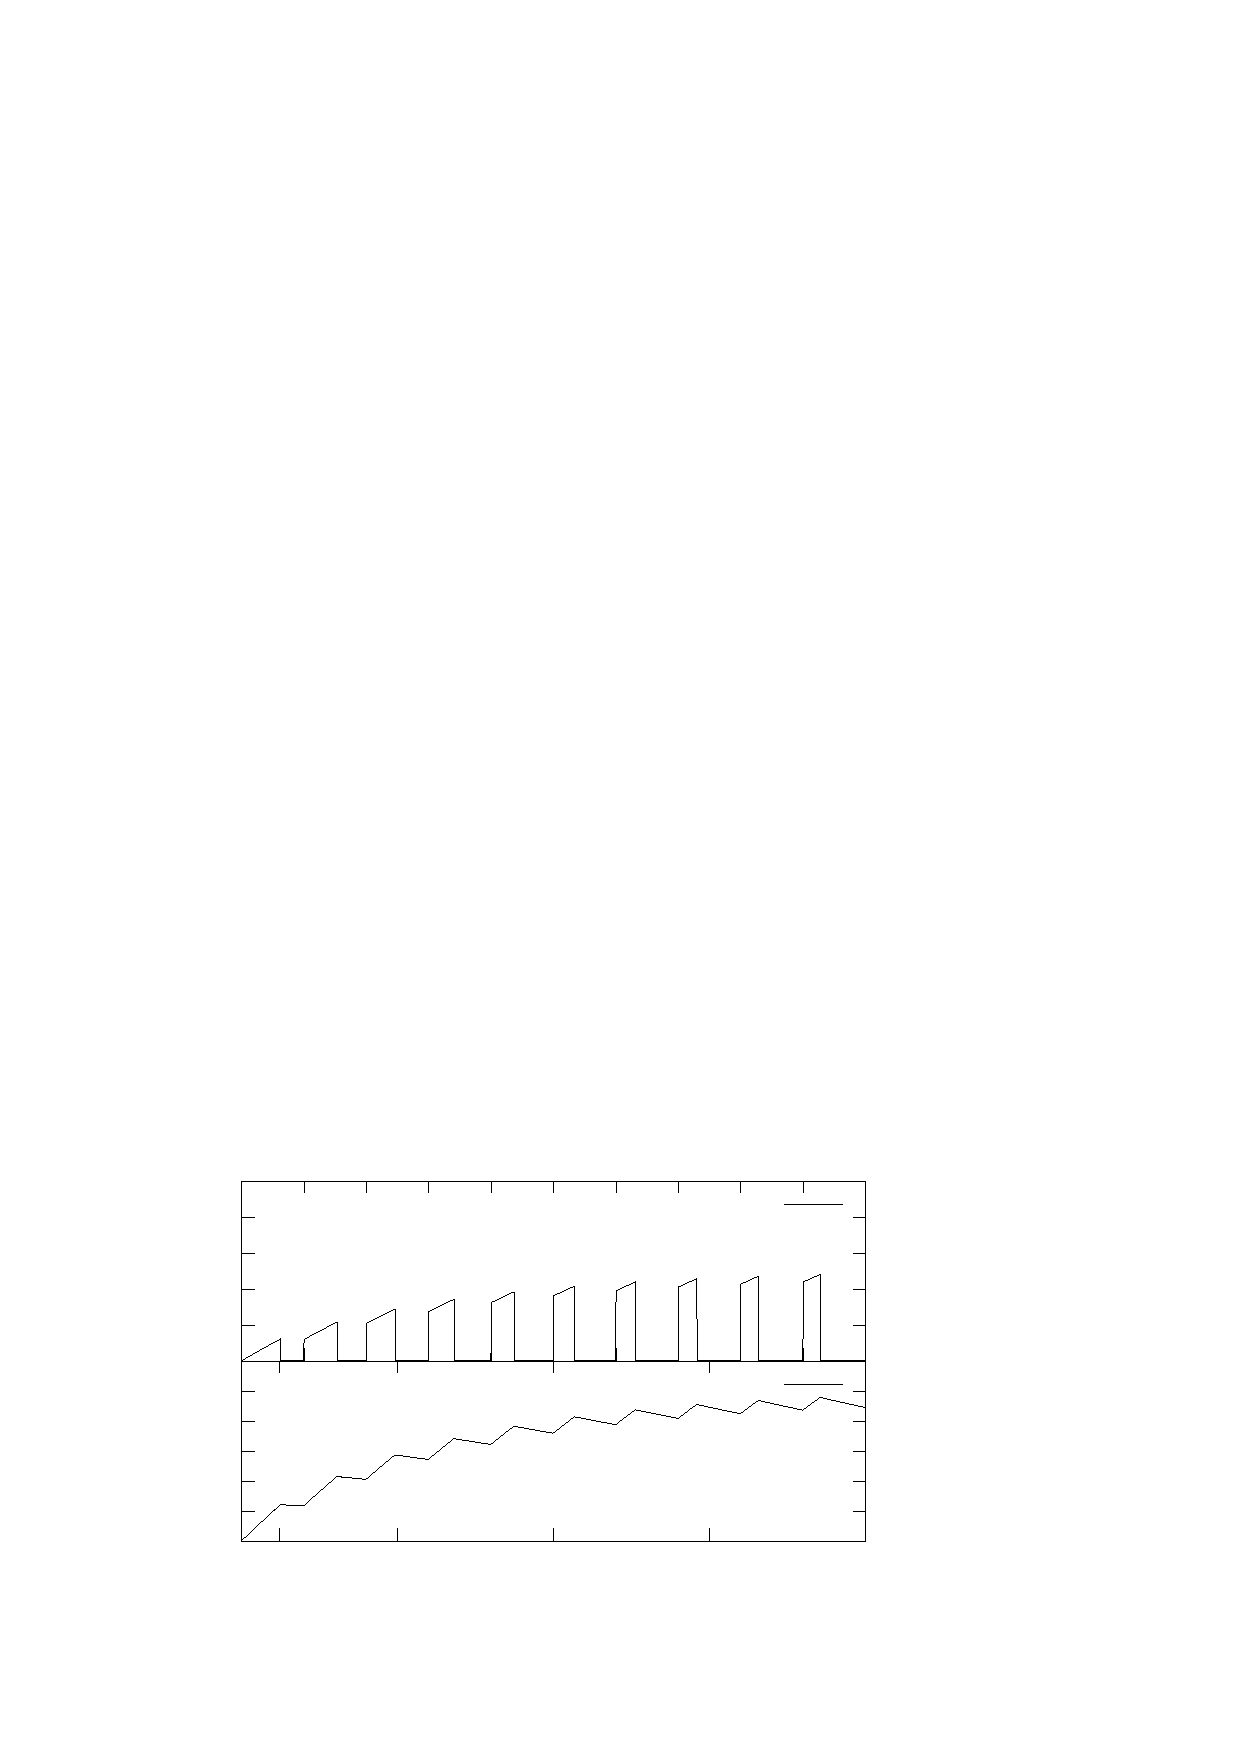
\includegraphics{CS_Siconos}%
\end{picture}%
\begingroup
\setlength{\unitlength}{0.0200bp}%
\begin{picture}(18000,10800)(0,0)%
\put(1925,5832){\makebox(0,0)[r]{\strut{} 0}}%
\put(1925,6696){\makebox(0,0)[r]{\strut{} 2}}%
\put(1925,7560){\makebox(0,0)[r]{\strut{} 4}}%
\put(1925,8424){\makebox(0,0)[r]{\strut{} 6}}%
\put(1925,9288){\makebox(0,0)[r]{\strut{} 8}}%
\put(1925,10152){\makebox(0,0)[r]{\strut{} 10}}%
\put(2200,5282){\makebox(0,0){\strut{}}}%
\put(3697,5282){\makebox(0,0){\strut{}}}%
\put(5195,5282){\makebox(0,0){\strut{}}}%
\put(6692,5282){\makebox(0,0){\strut{}}}%
\put(8190,5282){\makebox(0,0){\strut{}}}%
\put(9687,5282){\makebox(0,0){\strut{}}}%
\put(11185,5282){\makebox(0,0){\strut{}}}%
\put(12682,5282){\makebox(0,0){\strut{}}}%
\put(14180,5282){\makebox(0,0){\strut{}}}%
\put(15677,5282){\makebox(0,0){\strut{}}}%
\put(17175,5282){\makebox(0,0){\strut{}}}%
\put(550,7992){\rotatebox{90}{\makebox(0,0){\strut{}A}}}%
\put(14950,9577){\makebox(0,0)[r]{\strut{}$I_{s}$}}%
\put(1925,1512){\makebox(0,0)[r]{\strut{} 0}}%
\put(1925,2232){\makebox(0,0)[r]{\strut{} 1}}%
\put(1925,2952){\makebox(0,0)[r]{\strut{} 2}}%
\put(1925,3672){\makebox(0,0)[r]{\strut{} 3}}%
\put(1925,4392){\makebox(0,0)[r]{\strut{} 4}}%
\put(1925,5112){\makebox(0,0)[r]{\strut{} 5}}%
\put(1925,5832){\makebox(0,0)[r]{\strut{} 6}}%
\put(17175,962){\makebox(0,0){\strut{}2000}}%
\put(13429,962){\makebox(0,0){\strut{}1500}}%
\put(9684,962){\makebox(0,0){\strut{}1000}}%
\put(5938,962){\makebox(0,0){\strut{}500}}%
\put(3099,962){\makebox(0,0){\strut{}$t_s$}}%
\put(825,3672){\rotatebox{90}{\makebox(0,0){\strut{}V}}}%
\put(9687,137){\makebox(0,0){\strut{}time $micro$ s}}%
\put(14950,5257){\makebox(0,0)[r]{\strut{}$V_2$}}%
\end{picture}%
\endgroup
\endinput
}
  }\hspace{-2mm}
  \subfigure[{\sc Eldo} simulation ]  
  {\label{fig:ELDO_SIMU_CS} 
        \resizebox{0.5\linewidth}{!}{%GNUPLOT: LaTeX picture with Postscript
\begin{picture}(0,0)%
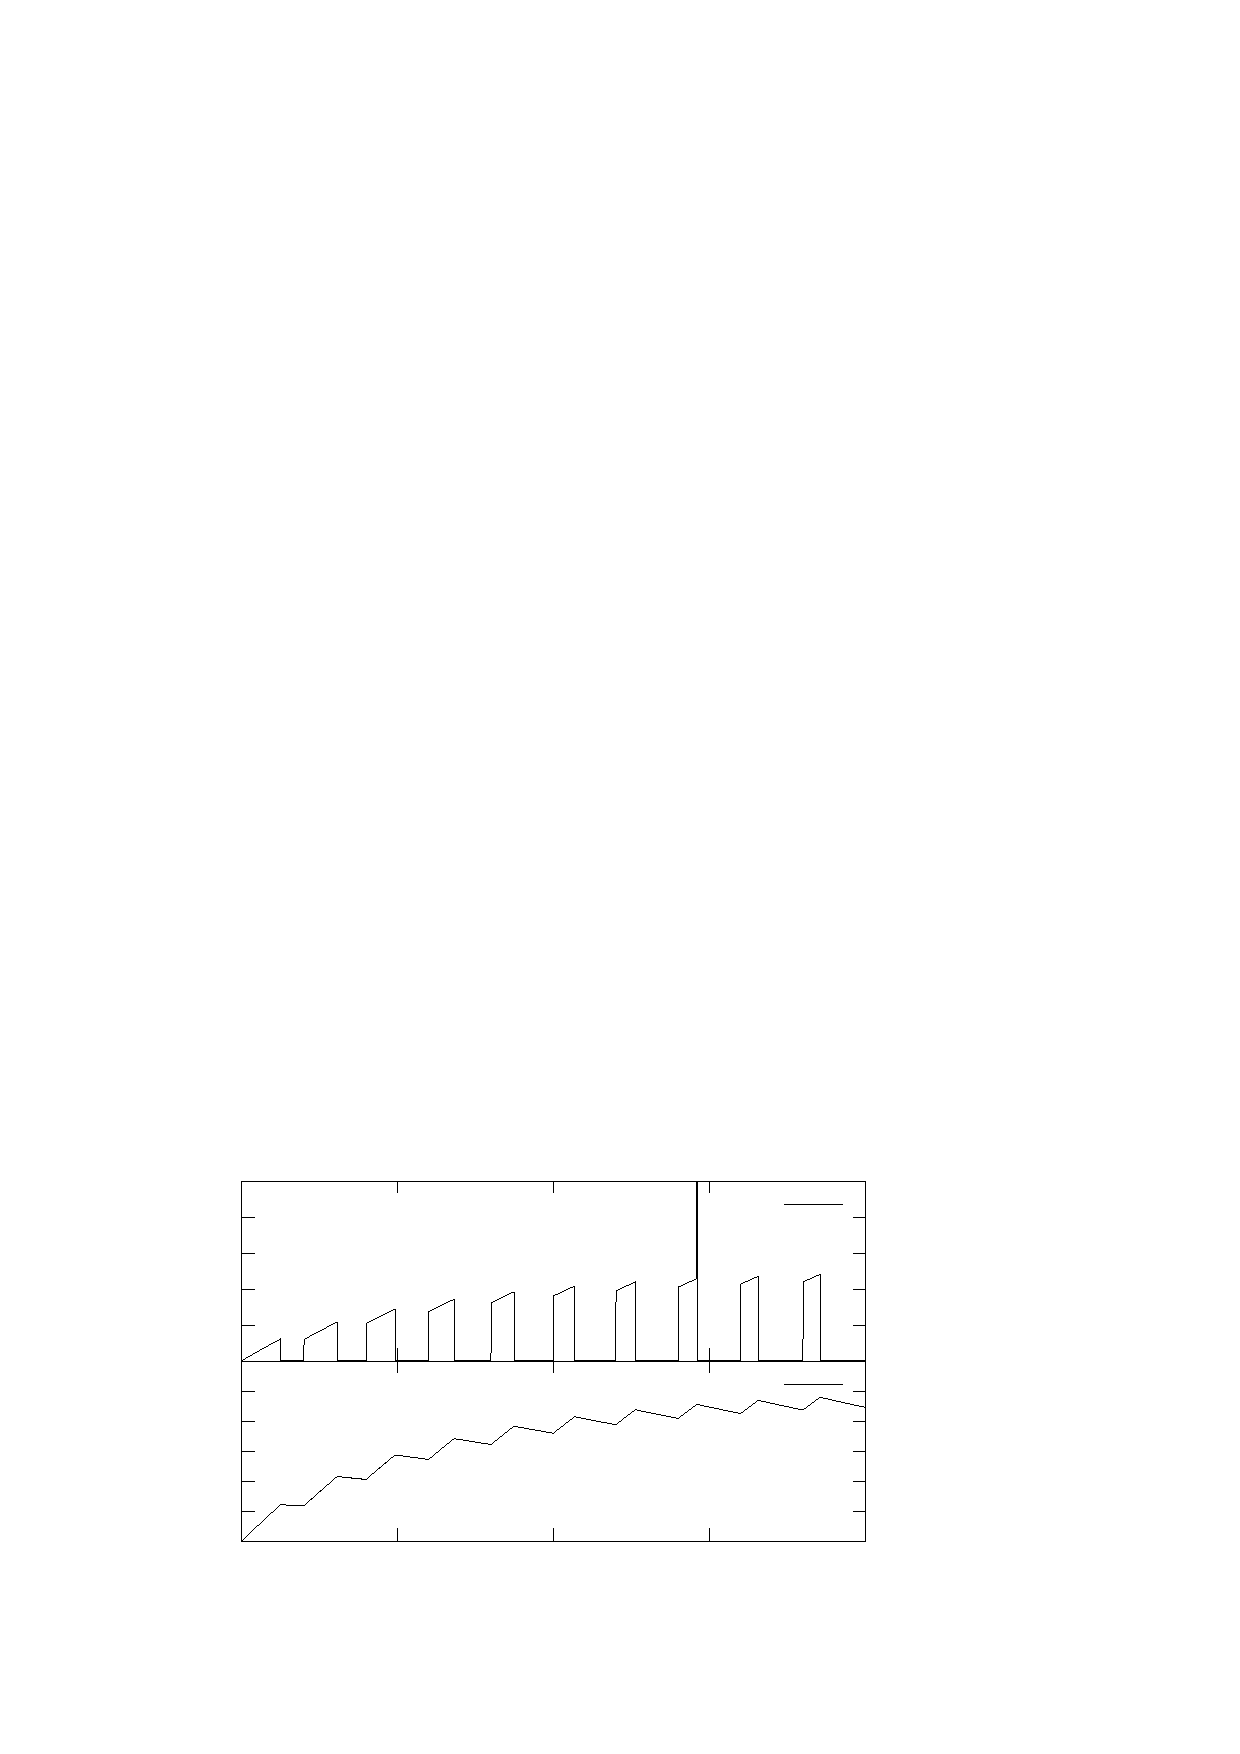
\includegraphics{eldo}%
\end{picture}%
\begingroup
\setlength{\unitlength}{0.0200bp}%
\begin{picture}(18000,10800)(0,0)%
\put(1925,5832){\makebox(0,0)[r]{\strut{} 0}}%
\put(1925,6696){\makebox(0,0)[r]{\strut{} 2}}%
\put(1925,7560){\makebox(0,0)[r]{\strut{} 4}}%
\put(1925,8424){\makebox(0,0)[r]{\strut{} 6}}%
\put(1925,9288){\makebox(0,0)[r]{\strut{} 8}}%
\put(1925,10152){\makebox(0,0)[r]{\strut{} 10}}%
\put(2200,5282){\makebox(0,0){\strut{}}}%
\put(5944,5282){\makebox(0,0){\strut{}}}%
\put(9687,5282){\makebox(0,0){\strut{}}}%
\put(13431,5282){\makebox(0,0){\strut{}}}%
\put(17175,5282){\makebox(0,0){\strut{}}}%
\put(550,7992){\rotatebox{90}{\makebox(0,0){\strut{}A}}}%
\put(14950,9577){\makebox(0,0)[r]{\strut{}$I_R$}}%
\put(1925,1512){\makebox(0,0)[r]{\strut{} 0}}%
\put(1925,2232){\makebox(0,0)[r]{\strut{} 1}}%
\put(1925,2952){\makebox(0,0)[r]{\strut{} 2}}%
\put(1925,3672){\makebox(0,0)[r]{\strut{} 3}}%
\put(1925,4392){\makebox(0,0)[r]{\strut{} 4}}%
\put(1925,5112){\makebox(0,0)[r]{\strut{} 5}}%
\put(1925,5832){\makebox(0,0)[r]{\strut{} 6}}%
\put(2200,962){\makebox(0,0){\strut{}0}}%
\put(5944,962){\makebox(0,0){\strut{}500}}%
\put(9687,962){\makebox(0,0){\strut{}1000}}%
\put(13431,962){\makebox(0,0){\strut{}1500}}%
\put(17175,962){\makebox(0,0){\strut{}2000}}%
\put(825,3672){\rotatebox{90}{\makebox(0,0){\strut{}V}}}%
\put(9687,137){\makebox(0,0){\strut{}time $micro$ s}}%
\put(14950,5257){\makebox(0,0)[r]{\strut{}$V_2$}}%
\end{picture}%
\endgroup
\endinput
}
  } 
 \caption{Switched circuit simulations.}
\label{figSimuCS}
\end{figure*}

\subsection{Numerical results with {\sc Eldo}}
{\sc Eldo} does not provide any non--smooth switch model. But it furnishes the 'VSWITCH' one described in
(\ref{eq:eldo_switch}), where  $R_S$ is the controlled resistor value of the switch, and $V_{C}$ the voltage
control. Setting $V_{\off}$ to $0$, and choosing a small value for $V_{\on}$ lead to: $R_S(t)=$
 \begin{equation}
    \label{eq:eldo_switch}
\begin{cases}R_\on\;  \mbox{if}\;V_{C}(t) \geq V_{\on},  \quad R_\off\;   \mbox{if}\;V_{C}(t) \leq
    V_{off} \\ (V_{C}(t)(R_\off\;-R_\on\;)+ R_\on\; V_{\off}- 
    R_\off\;V_{\on})/(V_{\off}-V_{\on})& \mbox{otherwise}\; \end{cases}
  \end{equation}
  which is close to \eqref{switchmodel1} for the chosen parameters. Simulations have been done using
  different sets of parameters. It is noteworthy that the
behavior of {\sc Eldo} depends on these values. For example, using a Backward Euler with the time step fixed to $0.1 \micro \second$ and $V_{on}=1e-4\volt$, $V_{off}=0 \volt$,
$R_\off\; = 1000 \ohm$, $R_\on\;=0.001\ohm$ cause troubles during the {\sc Eldo}
simulation, some messages like 'Newton no-convergence' appear. Fig.~\ref{fig:ELDO_SIMU_CS}
  shows the {\sc Eldo} simulation. The values are very close to the {\sc Siconos} simulation, except for the steps corresponding to the
  no-convergence messages. In this case, the resulting current value is absurd.
\section{Conclusions}
\label{section5}
{\color{navyblue}
In this paper it is  shown that Moreau's time-stepping scheme allows one to integrate an academic example on which Newton-Raphson based methods fail.  Comparisons with other analog simulators are presented.  This academic example demonstrates that analog tools can fail to simulate a switched circuit.
 Only a part of the advantages of the nonsmooth approach has been illustrated. More generally (see\cite{Acary.ea_RR2009}), it allows one to:
\begin{itemize}
\item avoid computing the dynamics changes due to topology variations, since the circuits are treated as a global system with a fixed state dimension; modes transitions are taken care of by the complementarity problem solvers, which usually are polynomial in time;
\item simulate circuits with very large number of events without slowing down too much the simulation;
\item avoid regularization and consequently stiff systems of ODEs;
\item accurately calculate the initial steady-state of the system;
\item accurately simulate sliding mode trajectories without spurious oscillations around the switching surface;
\item compute state jumps (initial jumps due to inconsistent states, or in the course of the integration). 
\end{itemize}
 
}



%%% Local Variables: 
%%% mode: latex
%%% TeX-master: "ISCASpaper"
%%% End: 
